\documentclass[class=report, crop=false, 12pt,a4paper]{standalone}
\usepackage{enumitem}
\usepackage{float}
\usepackage[normalem]{ulem}
\usepackage{graphicx}
\usepackage{amsmath}
\usepackage{siunitx}
\usepackage{commath}
\usepackage{tikz}
\usetikzlibrary{positioning, fit, calc}   
\tikzset{block/.style={draw, thick, text width=3cm ,minimum height=1.3cm, align=center},   
line/.style={-latex}     
}  
\begin{document}
\section{Tutorial Week 1: Continuity Equation}
\subsection{Exercise 2}
\subsubsection{Is the system steady?}
The system is steady due to the fact that our velocity field has no terms in $t$, meaning that our flow does not change with time - steady flow.
\subsubsection{Is the fluid incompressible?}
The fluid is compressible due to the fact that there is a $y$ component in the velocity field
\subsubsection{Make a vector map of the velocity field}
Using the following code, a vector field was mapped.
\begin{verbatim}
  %Hasha Dar

  [x,y]=meshgrid(-2:0.1:2,1:0.1:4); %field

  u = 0.*x; %x vector
  v = (4.*log(y) -2.*y + 10); %y vector

  quiver(x, y, u, v, 1) %plots quiver with arrow base at x, y 
  and direction u, v, scaling 1
\end{verbatim}
This produced the following plot:
\begin{figure}[H]
  \centering
  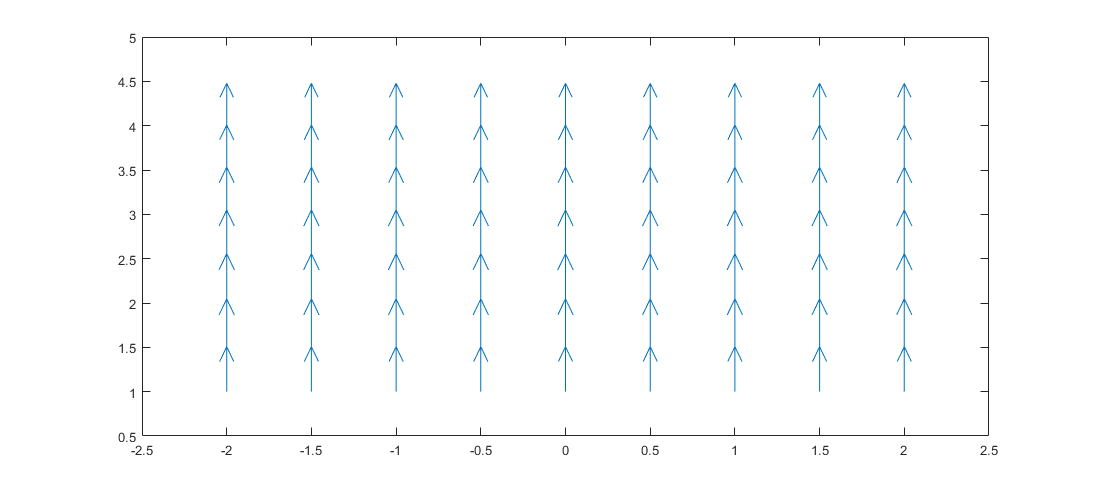
\includegraphics[width = \textwidth]{../img/quiverplotexercise20011-002.png}
\end{figure}
\subsubsection{Determine the variation of the volume dilatation rate in the flow domain}
\begin{gather}
  v = 4\ln{y} - 2y + 10\\
  \textrm{Volume dilatation} \rightarrow \frac{\partial v}{\partial y} = \frac{4}{y} - 2\\
  \textrm{Variation in volume dilatation} \rightarrow \frac{\partial ^2 v}{\partial y^2} = -\frac{4}{y^2}
\end{gather}
For the range $1 < y < 4$, the variation in the volume dilatation is negative, hence our fluid is compressible. 
\subsubsection{Estimate the volume dilatation rate in pints $(0, \ 1)$ and $(0, \ 3)$ of the flow domain}
\begin{gather}
  (0, \ 1) \rightarrow \frac{4}{1} - 2 = 2 \ \si{\per\second}\\
  (0, \ 3) \rightarrow \frac{4}{3} - 2 = -\frac{2}{3} \ \si{\per\second}
\end{gather}
\subsubsection{Sketch how a squared fluid parcel located in the points above would deform}
\end{document}